\begin{appendices}

\section{附录 A:单环马氏链速率函数 $I_J$ 的表达式 }{} \label{appendix:explicit} \label{appendix:explicit}
因此,可以得到速率函数:
\begin{equation*}\label{ratefunction2}
	\begin{split}
		I_J(\nu) =&\; \left[h\left(\nu^{12}\right)+h\left(\nu^{1N}\right)
		+h\left(\nu^+\right)+h\left(\nu^-\right)-h\left(\nu^{12}+\nu^{1N}+\nu^++\nu^-\right)\right] \\
		&\;+\inf_{X\in V(\nu)}F_{\nu}(X)+\sum_{i\in S}\left[ h\left(\nu_i-\nu^i\right)+h\left(\nu^i\right)
		-h\left(\nu_i\right)\right]-\sum_{c\in\mathcal{C}}\nu^c\log\gamma^c,
	\end{split}
\end{equation*}
下面将使用拉格朗日乘子法化简该式。固定 $\nu\in\mathcal{V}$,令拉格朗日函数 \cite{brian1990optimization} $\mathcal{A}_{\nu}:V(\nu)\times \mathbb{R}^{N-2}\to \mathbb{R}$ 为:
\begin{align*}
    \mathcal{A}_{\nu}(X,\lambda) = F_{\nu}(X) + \sum_{i=2}^{N-1} \lambda_i \left(x^{i} + y^{i} - \nu^{i,i+1}\right),
\end{align*}
其中 $X=(x^i,y^i)_{2\le i\le N-1}\in V(\nu)$ 并且 $\lambda=(\lambda_i)_{2\le i\le N-1}\in \mathbb{R}^{N-2}$。分别对 $x^{i}$,$y^{i}$ 和 $\lambda_i$求导,可以得到下列方程:
\begin{equation}\label{equation1}
	\begin{split}
		\log\left(x^{i}\right) - \log\left(x^{i-1}+x^{i}+\nu^{+}\right)  + \log\left(x^{i}+\nu^{+}\right) -\log\left(x^{i}+x^{i+1}+\nu^{+}\right)+\lambda_i  &= 0, \\
		\log\left(y^{i}+\nu^{-}\right) -\log\left(y^{i-1}+y^{i}+\nu^{-}\right)  + \log\left(y^{i}\right) - \log\left(y^{i}+y^{i+1}+\nu^{-}\right) +\lambda_i &= 0, \\
		x^{i} + y^{i} = \nu^{i,i+1},\qquad 2\le i\le N-1.\qquad\qquad\qquad
	\end{split}
\end{equation}
而且,可以把方程组 \eqref{equation1} 写为:
\begin{equation}\label{equations}
    \begin{split}
    \frac{x^{i}}{x^{i-1}+x^{i}+\nu^+}
    \,\frac{x^{i}+\nu^+}{x^{i}+x^{i+1}+\nu^+}
    &= \frac{y^{i}+\nu^-}{y^{i-1}+y^{i}+\nu^-}
    \,\frac{y^{i}}{y^{i}+y^{i+1}+\nu^-}=e^{-\lambda_i},\\
    x^{i} + y^{i} &= \nu^{i,i+1},\qquad 2\le i\le N-1.
    \end{split}
\end{equation}
其中 $x^1=\nu^{12}$,$x^N=0$,$y^1=0$ 和 $y^N=\nu^{1N}$。
    \begin{lemma}\label{lemma:existence for equations solution}
        方程 \eqref{equations} 有解 $X=(x^i,y^i)\in V(\nu)$。
    \end{lemma}
\begin{proof}
    若对某些 $2\le k\le N-1$ 存在 $\nu^{k,k+1}=0$,则有 $x^{k}=y^{k}=0$ 成立。那么依据指标 $2\le i\le k-1$ 和 $k+1\le i\le N-1$,方程 \eqref{equations} 可以被分为两个方程。因此对 $\nu^{k,k+1}>0, \forall k, 2\le k\le N-1$ 证明引理,下面会从三种不同情况考虑这个引理。

    情况 1:$\nu^{12}=\nu^{+}=\nu^{1N}=\nu^-=0$。
    易知,对每个 $\alpha\in (0,1)$,
    \begin{equation*}
        x^{i}=\alpha\nu^{i,i+1},\quad y^{i}=(1-\alpha)\nu^{i,i+1},\quad 2\le i\le N-1,
    \end{equation*}
    都是 \eqref{equations} 的解。

    情况 2:$\nu^{12}=\nu^{+}=0,\nu^{1N}+\nu^{-}>0$ 或 $\nu^{1N}=\nu^{-}=0,\nu^{12}+\nu^{+}>0$。容易验证若 $\nu^{12}=\nu^{+}=0,\nu^{1N}+\nu^{-}>0$成立,则$x^{i}=0,y^{i}=\nu^{i,i+1}$ 是方程 \eqref{equations} 的解。

    情况 3:$\nu^{12}+\nu^{+}>0$ 或 $\nu^{1N}+\nu^{-}>0$。上述已证明对任意给定的 $x^{k+1}\ge 0$,$y^{k+1}>0$,和 $x^{k+1}+y^{k+1}=\nu^{k+1,k+2}$,下列方程 \eqref{equations2} 满足 $x^{i},y^{i}> 0, \forall i, 2\le i\le k$。
    \begin{equation}\label{equations2}
        \begin{split}
            \frac{x^{i}}{y^{i}}
            =&\frac{x^{i}+x^{i+1}+\nu^+}{x^{i}+\nu^+}\, \frac{y^{i}+\nu^-}{y^{i-1}+y^{i}+\nu^-}
            \,\frac{x^{i-1}+x^{i}+\nu^+}{y^{i}+y^{i+1}+\nu^-},\\
            &\qquad x^{i} + y^{i} = \nu^{i,i+1},\qquad 2\le i\le k.
        \end{split}
    \end{equation}

    下面通过归纳法证明。若 $k=2$,方程 \eqref{equations2} 可以简化为:
    \begin{equation*}\label{equation k=2}
        \frac{x^{2}}{\nu^{23}-x^2}
        =\frac{x^{2}+x^{3}+\nu^+}{x^{2}+\nu^+}\, \frac{\nu^{12}+x^{2}+\nu^{+}}{\nu^{23}-x^2+y^3+\nu^-}.
        %,\qquad \nu^+_{23} + \nu^-_{23} = \nu_{23}.
    \end{equation*}
    易得:
    \begin{equation*}
        \lim_{x^{2}\downarrow 0}\frac{x^{2}}{\nu^{23}-x^2} = 0,\qquad \lim_{x^{2}\downarrow 0}\frac{x^{2}+x^{3}+\nu^+}{x^{2}+\nu^+}\, \frac{\nu^{12}+x^{2}+\nu^{+}}{\nu^{23}-x^2+y^3+\nu^-} \ge  \frac{\nu^{12}+\nu^{+}}{\nu^{23}+y^{3}+\nu^-} > 0.
    \end{equation*} 
    另外,
    \begin{equation*}
        \lim_{x^2\uparrow \nu^{23}}\frac{x^{2}}{\nu^{23}-x^2} = \infty,\qquad \lim_{x^{2}\uparrow \nu^{23}}\frac{x^{2}+x^{3}+\nu^+}{x^{2}+\nu^+}\, \frac{\nu^{12}+x^{2}+\nu^{+}}{\nu^{23}-x^2+y^3+\nu^-} =  \frac{\nu^{23}+x^{3}+\nu^+}{\nu^{23}+\nu^+}\frac{\nu^{12}+\nu^{23}+\nu^{+}}{y^{3}+\nu^-} < \infty.
    \end{equation*}
    通过中值定理,可以找到满足 $x^{i},y^i>0$ 的方程 \eqref{equations2} 的解,并且有 $x^{i}+y^{i}=\nu^{i,i+1}$ 。假设对 $k=n-1$ 命题成立,那么可以考虑方程:
    \begin{equation*}
        \frac{x^{n}}{\nu^{n,n+1}-x^{n}} = \frac{x^{n}+x^{n+1}+\nu^+}{x^{n}+\nu^+}\,\frac{\nu^{n,n+1}-x^{n}+\nu^-}{y^{n-1}+\nu^{n,n+1}-x^{n}+\nu^-}\,\frac{x^{n-1}+x^{n}+\nu^+}{\nu^{n,n+1}-x^{n}+y^{n+1}+\nu^-},
    \end{equation*}
    其中 $x^{n-1}$, $y^{n-1}$ 是方程 \eqref{equations2} 在 $k=n-1$ 时的解。可以得到:
    \begin{equation}\label{limit1}
        \lim_{x^{n}\downarrow 0}\frac{x^{n}}{\nu^{n,n+1}-x^{n}}=0,
    \end{equation}
    并且
    \begin{equation}\label{limit2}
        \begin{split}
            &\;\lim_{x^{n}\downarrow 0}\frac{x^{n}+x^{n+1}+\nu^+}{x^{n}+\nu^+}\,\frac{\nu^{n,n+1}-x^{n}+\nu^-}{y^{n-1}+\nu^{n,n+1}-x^{n}+\nu^-}\,\frac{x^{n-1}+x^{n}+\nu^+}{\nu^{n,n+1}-x^{n}+y^{n+1}+\nu^-}\\
            \ge &\;\frac{\nu^{n,n+1}+\nu^-}{\lim_{x^{n}\downarrow 0}(y^{n-1})+\nu^{n,n+1}+\nu^-}\,\frac{\lim_{x^{n}\downarrow 0}(x^{n-1})+\nu^+}{\nu^{n,n+1}+y^{n+1}+\nu^-}>0.
        \end{split}
    \end{equation}
    利用归纳法得出的结论 $\lim_{x^{n}\downarrow 0}(x^{n-1})>0$,可以得到下面两个式子成立。
    \begin{equation}\label{limit3}
        \lim_{x^{n}\uparrow \nu^{n,n+1}}\frac{x^{n}}{\nu^{n,n+1}-x^{n}}=\infty,
    \end{equation}
    和
    \begin{equation}\label{limit4}
        \begin{split}
            &\;\lim_{x^{n}\uparrow \nu^{n,n+1}}\frac{x^{n}+x^{n+1}+\nu^+}{x^{n}+\nu^+}\,\frac{\nu^{n,n+1}-x^{n}+\nu^-}{y^{n-1}+\nu^{n,n+1}-x^{n}+\nu^-}\,\frac{x^{n-1}+x^{n}+\nu^+}{\nu^{n,n+1}-x^{n}+y^{n+1}+\nu^-}\\
            \le &\;\frac{\nu^{n,n+1}+x^{n+1}+\nu^+}{\nu^{n,n+1}+\nu^+}\,\frac{\lim_{x^{n}\uparrow \nu^{n,n+1}}x^{n-1}+\nu^{n,n+1}+\nu^+}{y^{n+1}+\nu^-}<\infty.
        \end{split}
    \end{equation}
    那么通过中值定理,可以找到方程 \eqref{equations2} 满足条件 $x^{i},y^i>0, x^{i}+y^{i}=\nu^{i,i+1}, \forall i=2,3, \cdots, n$ 的解,就是说上述命题对 $k=n$ 成立。

    当 $k=N-1$ 时,有 $y^{k+1}=y^N=\nu^{1N}$ 成立。注意到 $\nu^{1N}+\nu^->0$,那么可以得到 \eqref{limit1},\eqref{limit2},\eqref{limit3} 和 \eqref{limit4} 成立。通过中值定理,可以找到方程 \eqref{equations2} 满足条件 $x^{i},y^i>0, x^{i}+y^{i}=\nu^{i,i+1}, \forall i=2,3, \cdots, n$ 的解。当 $k=N-1$ 时,方程 \eqref{equations2} 与 方程 \eqref{equations} 等价。证毕。

\end{proof}
\begin{lemma}\label{lemma:mininum}
    令 $X=(x^i,y^i)\in V(\nu)$ 是引理 ~\ref{lemma:existence for equations solution} 的解,那么 $X$ 是 $F_{\nu}(\cdot)$ 定义在 $V(\nu)$ 下的最小值点。 
\end{lemma}
\begin{proof}
    对任意 $a_1,a_2,b_1,b_2\ge 0$,通过 log-sum 不等式(见 \eqref{log sum inequality}),可以得到:
    \begin{align}\label{log sum inequality 2}
        a_1\log\frac{a_1}{a_1+a_2}+a_2\log\frac{a_2}{a_1+a_2}\ge a_1\log\frac{b_1}{b_1+b_2}+a_2\log\frac{b_2}{b_1+b_2}.
    \end{align}
    对任意 $Z=(z^i,w^i)\in V(\nu)$,可以把 \eqref{formula:F} 写为:
    \begin{align*}
        F_{\nu}(Z)
        =&\;\sum_{i=2}^{N-1}\left[ \left(z^{i-1}+\nu^+\right)\log\frac{z^{i-1}+\nu^+}{z^{i-1}+z^{i}+\nu^+} + z^{i}\log\frac{z^{i}}{z^{i-1}+z^{i}+\nu^+}  \right]\\
        &\;+\sum_{i=2}^{N-1}  \left[w^{i}\log\frac{w^{i}}{w^{i} +w^{i+1} +\nu^-} + \left(w^{i+1} +\nu^-\right)\log\frac{w^{i+1} +\nu^-}{w^{i} +w^{i+1} +\nu^-}\right],
    \end{align*}
    其中 $z^{1}=\nu^{12},w^{N}=\nu^{1N}$。再根据方程 \eqref{equations} 和 \eqref{log sum inequality 2}
    \begin{align*}
        F_{\nu}(Z)\ge &\;\sum_{i=2}^{N-1}\left[ \left(z^{i-1}+\nu^+\right)\log\frac{x^{i-1}+\nu^+}{x^{i-1}+x^{i}+\nu^+} + z^{i}\log\frac{x^{i}}{x^{i-1}+x^{i}+\nu^+}  \right]\\
        &\;+\sum_{i=2}^{N-1}  \left[w^{i}\log\frac{y^{i}}{y^{i} +y^{i+1} +\nu^-} + \left(w^{i+1} +\nu^-\right)\log\frac{y^{i+1} +\nu^-}{y^{i} +y^{i+1} +\nu^-}\right]\\
        =&\;\sum_{i=2}^{N-1}\left[ \nu^+\log\frac{x^{i-1}+\nu^+}{x^{i-1}+x^{i}+\nu^+} + z^{i}\log\frac{x^{i}+\nu^{+}}{x^{i-1}+x^{i}+\nu^{+}}\frac{x^{i}}{x^{i-1}+x^{i}+\nu^+}  \right]\\
        &\;+\sum_{i=2}^{N-1}  \left[\nu^-\log\frac{y^{i+1} +\nu^-}{y^{i} +y^{i+1} +\nu^-}+w^{i}\log\frac{y^{i}+\nu^{-}}{y^{i-1}+y^{i}+\nu^{-}}\frac{y^{i}}{y^{i} +y^{i+1} +\nu^-}  \right]\\
        &\;+\nu^{12}\log\frac{\nu^{12}+\nu^{+}}{\nu^{12}+x^{2}+\nu^{+}}+\nu^{1N}\log\frac{\nu^{1N}+\nu^{-}}{\nu^{1N}+y^{N-1}+\nu^{-}}\\
        =&\;\sum_{i=2}^{N-1}\left[-\lambda_i\nu^{i,i+1}+\nu^+\log\frac{x^{i-1}+\nu^+}{x^{i-1}+x^{i}+\nu^+}+\nu^-\log\frac{y^{i+1} +\nu^-}{y^{i} +y^{i+1} +\nu^-}\right]\\
        &\;+\nu^{12}\log\frac{\nu^{12}+\nu^{+}}{\nu^{12}+x^{2}+\nu^{+}}+\nu^{1N}\log\frac{\nu^{1N}+\nu^{-}}{\nu^{1N}+y^{N-1}+\nu^{-}}\\
        =&\;\sum_{i=2}^{N-1}\left[ \left(x^{i-1}+\nu^+\right)\log\frac{x^{i-1}+\nu^+}{x^{i-1}+x^{i}+\nu^+} + x^{i}\log\frac{x^{i}}{x^{i-1}+x^{i}+\nu^+}  \right]\\
        &\;+\sum_{i=2}^{N-1}  \left[y^{i}\log\frac{y^{i}}{y^{i} +y^{i+1} +\nu^-} + \left(y^{i+1} +\nu^-\right)\log\frac{y^{i+1} +\nu^-}{y^{i} +y^{i+1} +\nu^-}\right]\\
        =&\;F_{\nu}(X),
        \end{align*}
        其中 $\lambda_i$ 被表示为 \eqref{equations}。证毕。
\end{proof}

\section{速率函数的对称性} \label{appendix:symmetry}
下面将证明速率函数与初始分布的选择无关(见命题 \ref{corollary:rate function is unrelated to the starting state})。在开始证明之前,先给出下面的定义。

给定 $k=(k^c)_{c\in\mathcal{C}}\in \mathbb{N}^{2N+2}$ 和 $\eta=[i_0,i_1,\cdots,i_t]$,记 $|k|=\sum_{c\in\mathcal{C}}k^c|c|$,并且令 $n=|k|+|\eta|=|k|+t$,其中 $|c|$ 和 $|\eta|$ 分别表示环 $c$ 的长度和导出链的长度。令 $G^{\eta}(k)$ 为所有 $n$ 步长的轨道 $(\xi_m)_{0\le m\le n}$ 组成的集合,这些轨道满足环 $c$ 形成 $k^c$ 次,并且去环遗留的轨道是 $\eta$,定义为
\begin{equation*}
	G^{\eta}(k)=\left\{(\xi_0,\xi_1,\cdots,\xi_n)\in S^{n+1}:N^c_n=k^c (\forall c\in \mathcal{C}),\tilde{\xi}_n=\eta,\text{ and }n=|k|+|\eta|\right\}.
\end{equation*}
在此,对只有一个状态的 $\eta =[i]$,用 $G^{i}(k)$ 表示 $G^{\eta}(k)$。对任意包含状态 $i$ 的环 $\tilde{c}\in \mathcal{C}$,$G^i(k)$ 的一个子集 $G^{i,\tilde{c}}(k)$ 定义为:
\begin{equation*}
	G^{i,\tilde{c}}(k)=\left\{(\xi_0,\xi_1,\cdots,\xi_n)\in S^{n+1}:N^c_n=k^c (\forall c\in \mathcal{C}),\tilde{\xi}_n=[i],T^{\tilde{c}}_{k^{\tilde{c}}}=n,\text{ and }n=|k|\right\},
\end{equation*}
其中 $T^{\tilde{c}}_{k^{\tilde{c}}}$ 表示为第 $k^{\tilde{c}}$ 次形成的环 $\tilde{c}$。即对任意轨道 $(\xi_m)_{0\le m\le n}\in G^{i,\tilde{c}}(k)$,最后一次形成的环是 $\tilde{c}$。

注意到等式 $n=|k|+|\eta|$ 对 $G^{\eta}(k)$ 和 $G^{i,c}(k)$ 成立。因此在章节 ~\ref{LELDP} 省略 $G_n(k)$ 的角标 $n$。

下面将针对 $|G^i(k)|$ 和 $|G^{i,c}(k)|$,给出两个重要的等式。记 
\begin{equation*}
	B^i(\tilde{k})=\left|G^{i,+}(1,0,\tilde{k})\right|,\qquad	C^i(\tilde{k})=\left|G^{i,-}(0,1,\tilde{k})\right|,
\end{equation*}
其中 $\tilde{k}=(k^1,\cdots,k^N,k^{12},\cdots,k^{N-1,N},k^{1N})$,即 $B^i$ ($C^i$) 表示满足下列条件的轨迹数量:1)环 $c$ 形成 $k^c$ 次;2) $k^+=1,k^-=0$ ($k^+=0,k^-=1$);3)从状态 $i$ 出发,状态 $i$ 结束;4)最后形成的环是 $(1,\cdots,N)$ ($(1,N,\cdots,2)$)。

\begin{lemma}\label{lemma:BiBjCiCj}
	对任意 $i,j\in S$,有:
	\begin{equation*}
		B^i\left(\tilde{k}\right)=B^j\left(\tilde{k}\right)=C^i\left(\tilde{k}\right)=C^j\left(\tilde{k}\right).
	\end{equation*}
\end{lemma}

\begin{proof}
    不降低一般性,令 $i=1$,只须证 $B^1(\tilde{k})=C^1(\tilde{k})=B^j(\tilde{k})$。

    首先证明 $B^1(\tilde{k})=C^1(\tilde{k})$。
    \begin{figure}[h]
		\centering
		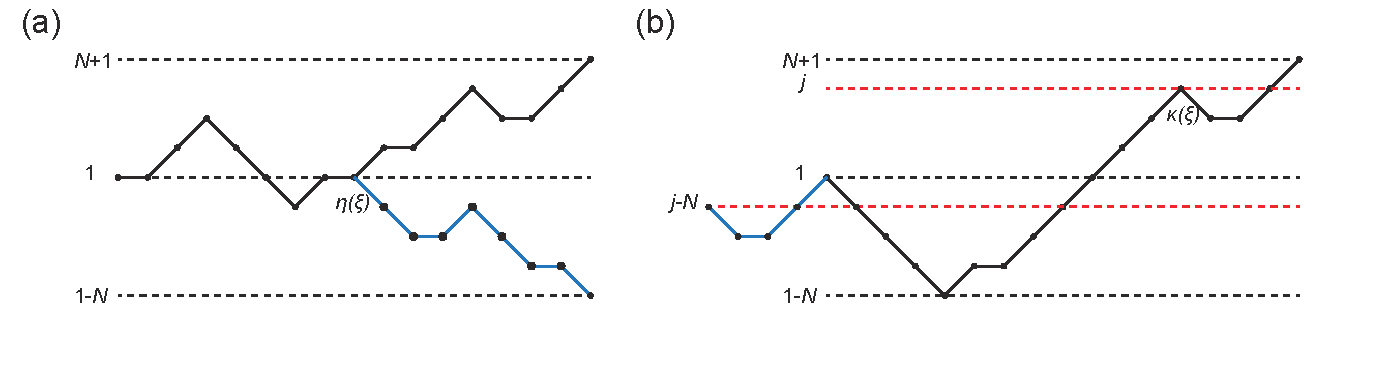
\includegraphics[scale=0.7]{chart/brokenlinegraph.pdf}
		\caption{$\xi$ 的轨迹对应的折线图。(a)第一种类型的轨迹映射(b)第二种类型的轨迹映射}
		\label{fig:linechart}
	\end{figure}
    注意到该系统是单环马氏链,$\xi$ 的每条轨迹可以被看作是一个折线图(见图 \ref{fig:linechart}(a))折线在状态 $i$ 时间 $m$ 处的水平移动表示环 $(i)$ 在时间 $m$ 处形成。折线从状态$i+1$ ($-j$) 到状态 $i$ ($1-j$) 的每次上升对应于 (其中的加减运算的结果都会经过模 $N$ 运算)。对任意轨迹 $\xi=(\xi_m)_{0\le m\le n}\in G^{1,+}(1,0,\tilde{k})$,令 $\eta(\xi)=\max\{m: 0\le m\le n-1,\xi_m=1\}$。回顾定义 $G^{1,+}(1,0,\tilde{k})$,轨迹 $(\xi_m)_{0\le m\le n}$ 在时间 $n$ 和状态 $N+1$ 到达集合 $\{N+1,1-N\}$。那么构造 $\xi$ 对应的轨迹 $\tilde{\xi}$(见图 \ref{fig:linechart} (a))
	\begin{equation*}
		\tilde{\xi}_m
		:=\left\{\begin{aligned}
			&\xi_m,    && \text{if } 0\le m\le \eta(\xi),\\
			&\xi_{n+\eta(\xi)-m},    && \text{if }\eta(\xi)<m\le n.\\
		\end{aligned}\right.
	\end{equation*}
    所有 $(\xi_m)_{0\le m\le \eta(\xi)}$ 中形成的环,在$(\tilde{\xi}_m)_{0\le m\le \eta(\xi)}$中也有形成。折线轨迹 $(\xi_m)_{\eta(\xi)\le m\le n}$ 在状态 $i$ 时间 $m$ 的水平移动对应于 $(\tilde{\xi}_m)_{\eta(\xi)\le m\le n}$ 在状态 $i-N$ 时间 $n+\eta(\xi)-m$ 的水平移动。类似的,折线轨迹 $(\xi_m)_{\eta(\xi)\le m\le n}$ 在时间 $m$ 从状态$i+1$ 到状态 $i$ 的下落对应于 $(\tilde{\xi}_m)_{\eta(\xi)\le m\le n}$ 在时间 $n+\eta(\xi)-m$ 从状态 $i-N$ 到状态 $i+1-N$ 的下落。那么所有 $(\xi_m)_{0\le m\le \eta(\xi)}$中形成的单状态和两状态环在 $(\tilde{\xi}_m)_{0\le m\le \eta(\xi)}$ 中也有对应。而且,轨迹 $(\tilde{\xi}_m)_{0\le m\le n}$ 在时间 $n$ 和状态 $1-N$第一次到达集合 $\{N+1,1-N\}$,这说明轨迹 $(\tilde{\xi}_m)_{0\le m\le n}$ 最后形成的环是 $(1,N,\cdots,2)$,使得 $\tilde{\xi}\in G^{1,-}(0,1,\tilde{k})$。那么 $\xi\to \tilde{\xi}$ 是从 $G^{1,+}(1,0,\tilde{k})$ 到 $G^{1,-}(0,1,\tilde{k})$ 的一一映射,这说明 $B^1(\tilde{k})=C^1(\tilde{k})$。

    现在已经证明 $B^1(\tilde{k})=B^j(\tilde{k})$。对任意 $\tilde{k}$,令 $\tilde{G}^i(\tilde{k})$ 为满足下列所有条件路径的集合,1)前 $n$ 步($n=N+\sum_{i \in S}(k^i+2k^{i,i+1})$)是从状态 $i$ 出发。2)边 $\langle i,i\rangle$ 被通过 $k^i$ 次。3)边 $\langle i,i+1\rangle$ 被通过 $k^{i,i+1}$ 次。4)在时间 $n$ 第一次到达状态 $N+i$。

    已经阐明对任意 $j\in S$,$|\tilde{G}^1(\tilde{k})|=|\tilde{G}^j(\tilde{k})|$ 成立。对任意轨迹 $\xi=(\xi_m)_{0\le m\le n}\in \tilde{G}^{1}(\tilde{k})$,令 $\kappa^j(\xi)=\min\{m: 0\le m\le n,\xi_k=j\}$,$\xi$也可以被视为折线图(见图 \ref{fig:linechart} (b))。那么构造 $\xi$ 对应的轨迹 $\tilde{\xi}$ 为:
    \begin{equation*}
		\tilde{\xi}_k
		:=\left\{\begin{aligned}
			&\xi_{\kappa(\xi)+k},    && \text{if } 0\le k\le n-\kappa(\xi),\\
			&\xi_{k+\kappa(\xi)-n},    && \text{if }n-\kappa(\xi)<k\le n.\\
		\end{aligned}\right.
	\end{equation*}
    因此 $(\tilde{\xi}_m)_{0\le m\le n} \in \tilde{G}^i(\tilde{k})$。注意到 $\kappa(\xi)$ 是 $\xi$ 第一次到达状态 $j$,这说明 $n$ 也是 $\tilde{\xi}$ 第一次到达状态 $j+N$,那么$\tilde{\xi}\in \tilde{G}^j(\tilde{k})$。显然,$\xi\to\tilde{\xi}$ 是从 $\tilde{G}^1(\tilde{k})$ 到 $\tilde{G}^j(\tilde{k})$的一一映射,这说明 $|\tilde{G}^1(\tilde{k})|=|\tilde{G}^j(\tilde{k})|$。

    对轨迹 $\xi\in\tilde{G}^j(\tilde{k})$,环 $(i)$,$(i,i+1)$,$(1,\cdots,N)$,$(1,N,\cdots,2)$ 分别形成 $k^i$,$k^{i,i+1}-l$,$l+1$,$l$ 次,其中 $l\le \min_{i\in S}k^{i,i+1}$ 依赖于 $\xi$。注意到 $\xi$ 在 $n$ 时到达状态 $N+j$ ,那么 $\xi$ 形成的最后一个环是 $(1,\cdots,N)$,因此
	\begin{equation*}
		\tilde{G}^j\left(\tilde{k}\right)=\bigsqcup_{l=0}^{\min_{i\in S}k^{i,i+1}}G^{j,+}\left(l+1,l,k^1,\cdots,k^N,k^{12}-l,\cdots,k^{N1}-l\right),
	\end{equation*}
	\begin{equation}\label{equality for AjBj}
		\left|\tilde{G}^j\left(\tilde{k}\right)\right|=\sum_{l=1}^{\min_{i\in S}k^{i,i+1}}\left|G^{j,+}\left(l+1,l,k^1,\cdots,k^N,k^{12}-l,\cdots,k^{N1}-l\right)\right|+B^j\left(\tilde{k}\right).
	\end{equation}
	下面用归纳法证明 $B^1(\tilde{k})=B^j(\tilde{k})$。当 $\min_{i\in S}k^{i,i+1}=0$, 通过方程 \eqref{equality for AjBj},可以得到 
    \begin{equation*}
		B^1(\tilde{k})=|\tilde{G}^1(\tilde{k})|=|\tilde{G}^j(\tilde{k})|=B^j(\tilde{k}).
	\end{equation*} 
	假设等式对 $\min_{i\in S}k^{i,i+1}\le m$ 成立。当 $\min_{i\in S}k^{i,i+1}=m+1$ 时,固定 $1\le l\le \min_{i\in S}k^{i,i+1}$,并且令 $\xi\in G^{j,+}_n(l+1,l,k^1,\cdots,k^N,k^{12}-l,\cdots,k^{N1}-l)$。那么轨迹 $\xi$ 可以被分为 $2l+1$ 个子轨迹, 是的每一个子轨迹最后形成的环是 $(1,\cdots,N)$ 或 $(1,N,\cdots,2)$。Note that the number of permutations for inserting $l$ cycle $(1,\cdots,N)$ and $l$ cycle $(1,N,\cdots,2)$ into state 1 before the last cycle $(1,\cdots,N)$ is $\binom{2l}{l}$. Fix the partition of the rest cycles (i.e. $\sum_{s=1}^{2l+1}\tilde{k}_s=(k^1,\cdots,k^N,k^{12}-l,\cdots,k^{N1}-l)$), as $B^{i}(\tilde{k})=C^i(\tilde{k})$ for all $i$ and $\tilde{k}$, the number of insertions is $\prod_{s=1}^{2l+1}B^j(\tilde{k}_s)$, so that
	\begin{align*}
		&\;\left|G^{j,+}\left(l+1,l,k^1,\cdots,k^N,k^{12}-l,\cdots,k^{N1}-l\right)\right|\\
		=&\;\binom{2l}{l}\sum_{\sum_{s=1}^{2l+1}\tilde{k}_s=(k^1,\cdots,k^N,k^{12}-l,\cdots,k^{N1}-l)}\prod_{s=1}^{2l+1}B^j\left(\tilde{k}_s\right).
	\end{align*}
	As $l\ge 1$, we have $B^1(\tilde{k}_s)=B^j(\tilde{k}_s)$, so that
	\begin{align*}
		&\left|G^{1,+}\left(l+1,l,k^1,\cdots,k^N,k^{12}-l,\cdots,k^{N1}-l\right)\right|\\
		=&\left|G^{j,+}\left(l+1,l,k^1,\cdots,k^N,k^{12}-l,\cdots,k^{N1}-l\right)\right|.
	\end{align*}
	Then by the claim and \eqref{equality for AjBj}, we have $B^1(\tilde{k})=B^j(\tilde{k})$. By induction, we finish the proof.
\end{proof}
\begin{proposition}\label{proposition:E Gin}
	For any $1\le i,j\le N$, $k\in\mathbb{N}^{2N+2}$, and derived chain $\eta$,
	\begin{itemize}
		\item[(i)] 
		\begin{equation}\label{EGin}
			\left|G^i\left(k^+,k^-,\tilde{k}\right)\right|=\left|G^i\left(k^-,k^+,\tilde{k}\right)\right|.
		\end{equation}
		\item[(ii)] 
		\begin{equation}\label{E Gi1cdotsNn}
			\left|G^{i,+}(k)\right|=\left|G^{j,+}(k)\right|,\qquad\left|G^{i,-}(k)\right|=\left|G^{j,-}(k)\right|.
		\end{equation}
		\item[(iii)]  
		\begin{equation}\label{EGetan}
			\left|G^{\eta}\left(k^+,k^-,\tilde{k}\right)\right|=\left|G^{\eta}\left(k^-,k^+,\tilde{k}\right)\right|.
		\end{equation}
	\end{itemize}
\end{proposition}
\begin{proof}
	(i) We first insert $k^+$ cycle $(1,\cdots,N)$ and $k^-$ cycle  $(1,N,\cdots,2)$ into state $i$, then the number of permutations is $\binom{k^++k^-}{k^+}$. 
	
	We next divide the rest cycles (i.e. $k^i$ cycle $(i)$ and $k^{i,i+1}$ cycle $(i,i+1)$) into $k^++k^-+1$ parts. Fix the partition of the rest cycles as $\sum_{s=1}^{k^++k^-+1}\tilde{k}_s=\tilde{k}$. By Lemma~\ref{lemma:BiBjCiCj},  the number of insertions is 
	\begin{equation*}
		\left[\prod_{s=1}^{k^++k^-}B^i(\tilde{k}_s)\right]\left|G^i(0,0,\tilde{k}_{k^++k^-+1})\right|,
	\end{equation*}
	where $B^i(\tilde{k}_s)$ is the number of the insertion of $\tilde{k}_s$ cycles between the $(s-1)$-th and $s-$th long $N$-state cycle, and $|G^i(0,0,\tilde{k}_{k^++k^-+1})|$ is the number of the insertion of $\tilde{k}_{k^++k^-+1}$ cycles after the $(k^++k^-)$-th long $N$-state cycle. Adding the number of the insertions over all partitions $\sum_{s=1}^{k^++k^-+1}\tilde{k}_s=\tilde{k}$, we have
	\begin{align}\label{E Gin}
		\left|G^i\left(k^+,k^-,\tilde{k}\right)\right|=\binom{k^++k^-}{k^+}\sum_{\sum_{s=1}^{k^++k^-+1}\tilde{k}_s=\tilde{k}}\left[\prod_{s=1}^{k^++k^-}B^i\left(\tilde{k}_s\right)\right]\left|G^i\left(0,0,\tilde{k}_{k^++k^-+1}\right)\right|.
	\end{align}
	Note that \eqref{E Gin} is symmetry about $k^+$ and $k^-$, we finish the proof of (i).
	
	(ii) We only prove the first equality of \eqref{E Gi1cdotsNn} and the second equality is similar. The proof is similar with (i), but here for trajectory $\xi\in G^{i,+}_n(k)$, the last cycle is $(1,\cdots,N)$, we only need to insert $k^+-1$ cycle $(1,\cdots,N)$ and $k^-$ cycle $(1,N,\cdots,2)$ into state $i$, then we have
	\begin{align*}
		&\left|G^{i,+}\left(k\right)\right|=\binom{k^++k^--1}{k^+-1}\sum_{\sum_{s=1}^{k^++k^-}\tilde{k}_s=\tilde{k}}\prod_{s=1}^{k^++k^-}B^i\left(\tilde{k}_s\right)\\
		&\qquad\qquad=\binom{k^++k^--1}{k^+-1}\sum_{\sum_{s=1}^{k^++k^-}\tilde{k}_s=\tilde{k}}\prod_{s=1}^{k^++k^-}B^j\left(\tilde{k}_s\right)=\left|G^{j,+}\left(k\right)\right|,
	\end{align*}
	where the second equality follows from Lemma~\ref{lemma:BiBjCiCj}.
	
	(iii) Let $\eta=[i_0,i_1,\cdots,i_t]$. We first divide all cycles into $t+1$ parts. Fix a partition as $\sum_{s=0}^t k_s=k$, so that $k^c_s$ cycle $c$ ($\forall c\in\mathcal{C}$) will be inserted into state $i_s$ ($0\le s\le t$) of $\eta$. Then the number of insertions is $\prod_{s=0}^t |G^{i_s}(k_s)|$. Adding the number of insertions over all partitions $\sum_{s=0}^t k_s=k$, we have
	\begin{equation*}
		\left|G^{\eta}(k)\right|=\sum_{\sum_{s=0}^t k_s=k}\prod_{s=0}^t \left|G^{i_s}(k_s)\right|.
	\end{equation*}
	Note that for any partition $\sum_{s=0}^t k_s=k$, we have $\sum_{s=0}^t (k_s^-,k_s^+,\tilde{k}_s)=(k^-,k^+,\tilde{k})$ is a partition for $(k^-,k^+,\tilde{k})$. Then by Eq. \eqref{EGin}, we have
	\begin{align*}
		\left|G^{\eta}(k^-,k^+,\tilde{k})\right|=&\sum_{\sum_{s=0}^t (k_s^-,k_s^+,\tilde{k}_s)=(k^-,k^+,\tilde{k})}\prod_{s=0}^t \left|G^{i_s}(k_s^-,k_s^+,\tilde{k}_s)\right|\\
		=&\sum_{\sum_{s=0}^t k_s=k}\prod_{s=0}^t \left|G^{i_s}(k_s)\right|=\left|G^{\eta}(k)\right|.
	\end{align*}
\end{proof}
Next statement, we give a relation between $| (G^i(k)|$ and $|G^{i,c}(k)|$.
\begin{lemma}\label{lemma:E G1cnk}
	For any $k\in \mathbb{N}^{2N+2}$ and $i\in S$, let $c\in \mathcal{C}$ satisfies $c$ passing through state $i$, then
	\begin{align*}
		\left|G^{i,c}(k)\right| = \frac{k^c}{k_i}\left|G^i(k)\right|.
	\end{align*}
\end{lemma}
\begin{proof}
	Without loss of generality, we only prove for $i=1$. Recall that the three steps of calculation for $|G^1(k)|$ in Section~\ref{LELDP}. 
%	let us insert cycle $(1)$ earlier from the third step to the first step, then $A_1$ and $A_3$ turn into
%	\begin{equation*}
%		\hat{A}_1=\binom{k^1+k^{12}+k^{1N}+k^{+}+k^{-}}{k^1, k^{12}, k^{1N}, k^{+}, k^{-}},\qquad \hat{A}_3=\prod_{i=2}^N \binom{\sum_{c \ni \{i\}} k^{c} - 1}{ k^{i} },
%	\end{equation*}
%	and it is easy to check $A_1A_3=\hat{A}_1\hat{A}_3$.
%	
	Let us fix the last cycle as $c$ in the first step and the number of permutations is turning into
	\begin{equation*}
		\frac{k^c}{k^{1}+k^{12}+k^{1N}+k^{+}+k^{-}}A_1.
	\end{equation*}
	Keep the second step and the third step the same. In this case the last cycle formed by trajectory will be $c$, which means
	\begin{align*}
		\left|G^{1,c}(k)\right| = \frac{k^c}{k_1}\left|G^1(k)\right|.
	\end{align*}
\end{proof}
\begin{proposition}\label{corollary:rate function is unrelated to the starting state}
	$I_J$ is independent of the choice of the initial distribution of $\xi$.
\end{proposition}
\begin{proof}
	Let $c=(1,\cdots,N)$ or $(1,N,\cdots,2)$, by Proposition~\ref{proposition:E Gin} and Lemma~\ref{lemma:E G1cnk}, it is easy to see that $\log|G^1(k)|=\log|G^i(k)|+O(\log n)$. Then by \eqref{ratefunction}, we finish the proof.
\end{proof}


\end{appendices}
